\documentclass{standalone}
\usepackage{tikz}
\usetikzlibrary{patterns, positioning}
\usepackage[sfdefault]{ClearSans} %% option 'sfdefault' activates Clear Sans as the default text font
\usepackage[T1]{fontenc}

\begin{document}
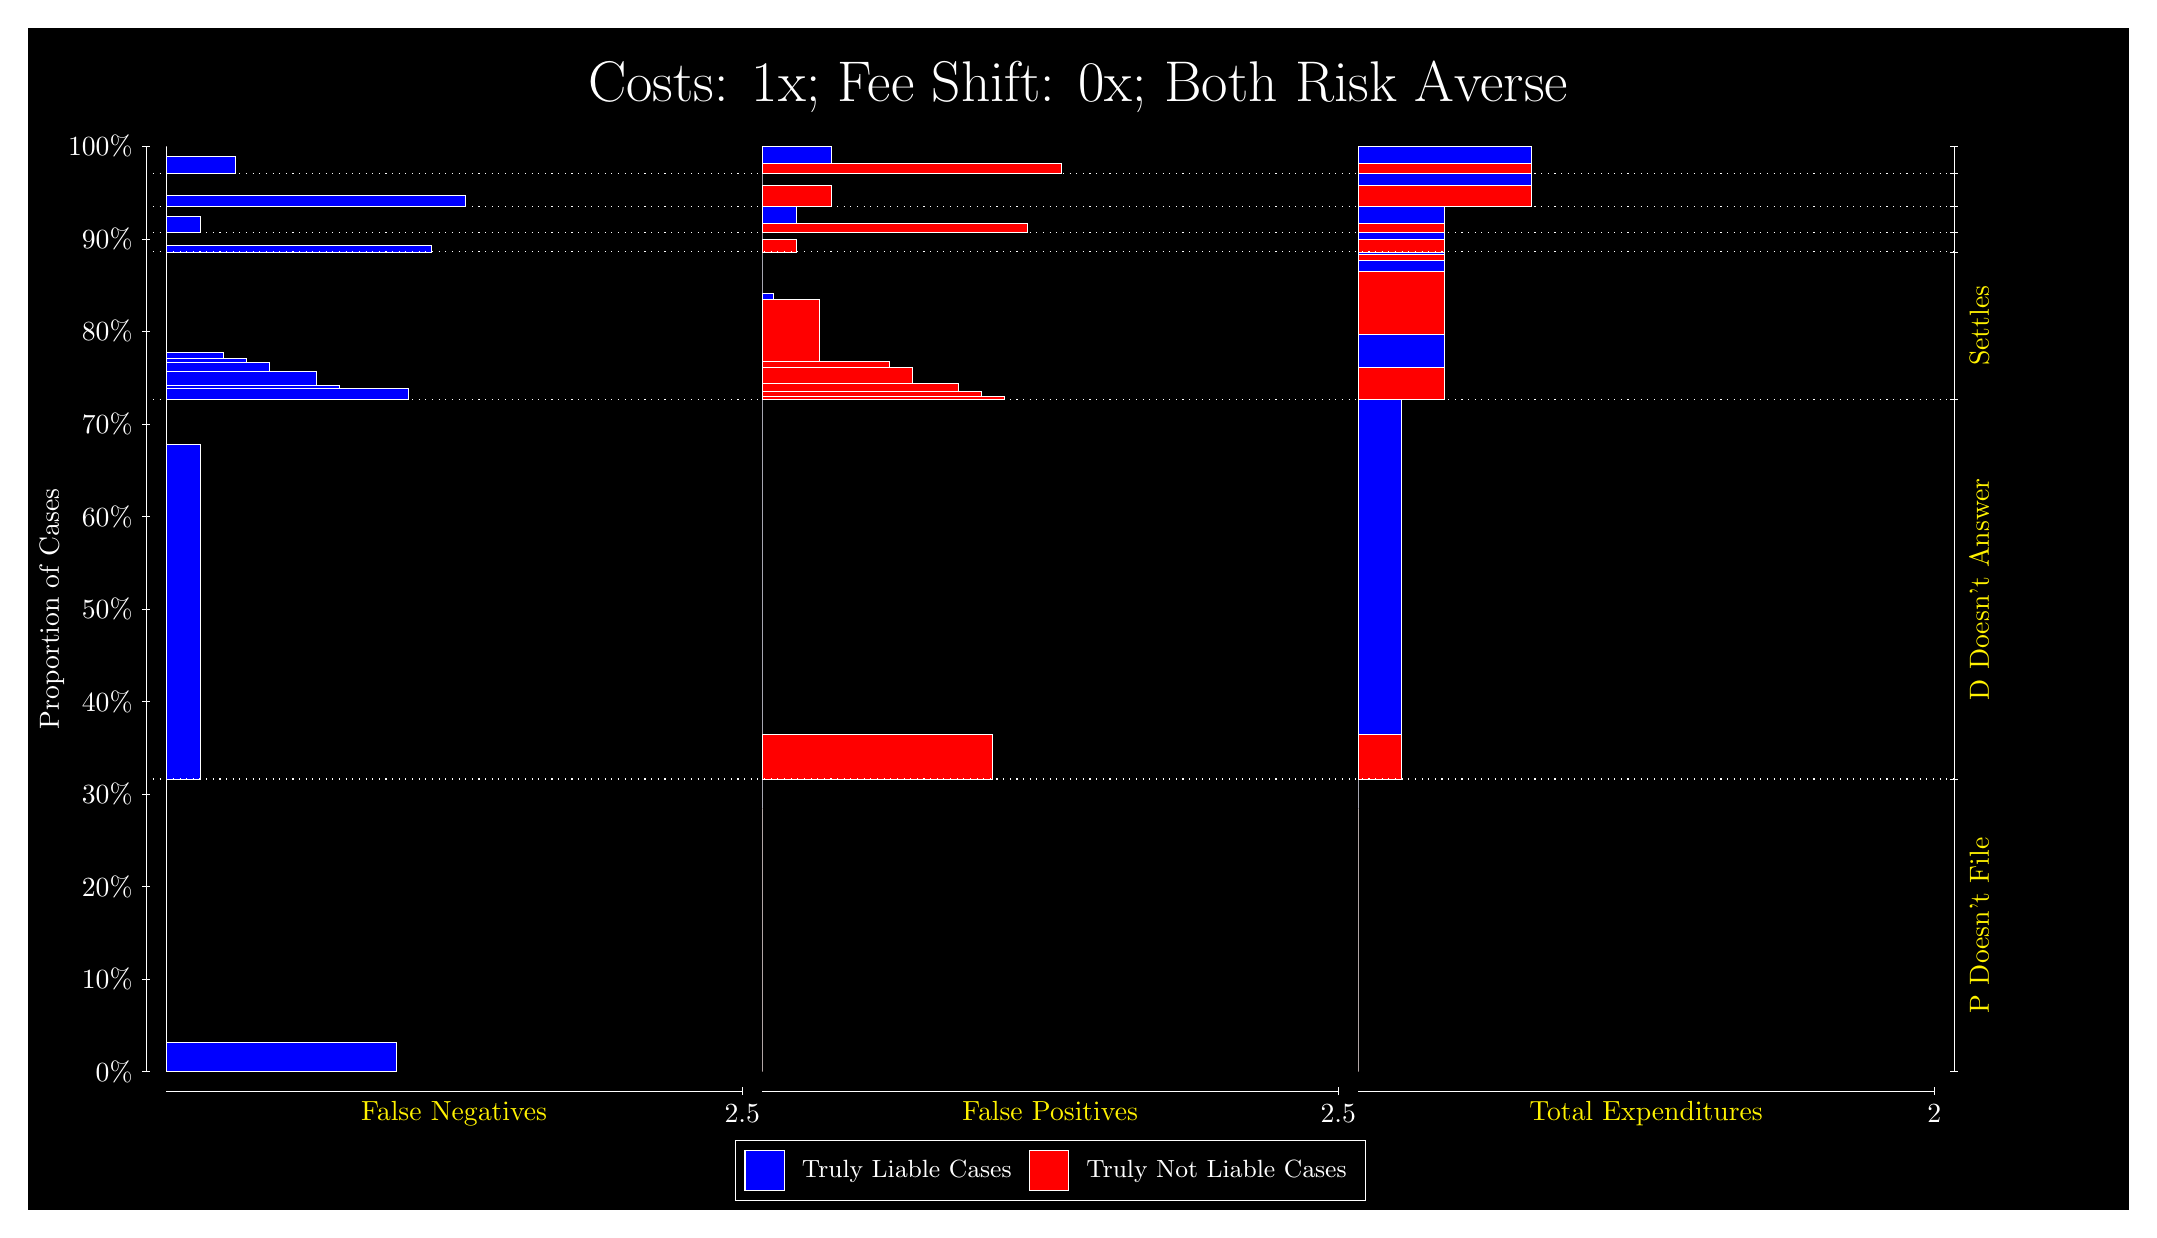
\begin{tikzpicture}
\draw[fill=black] (0,0) rectangle (26.667,15);
\draw[text=white] (0,13.5) rectangle (26.667,15) node[midway] {\huge Costs: 1x; Fee Shift: 0x; Both Risk Averse};
\draw[white, very thin] (1.5,1.75) -- (1.5,13.5);
\node[rotate=90, text=white, anchor=center] at (0.3, 7.625) {Proportion of Cases};
\draw[white, very thin] (1.45,1.75) -- (1.55,1.75);
\node[text=white, anchor=east] at (1.45, 1.75) {0\%};
\draw[white, very thin] (1.45,2.925) -- (1.55,2.925);
\node[text=white, anchor=east] at (1.45, 2.925) {10\%};
\draw[white, very thin] (1.45,4.1) -- (1.55,4.1);
\node[text=white, anchor=east] at (1.45, 4.1) {20\%};
\draw[white, very thin] (1.45,5.275) -- (1.55,5.275);
\node[text=white, anchor=east] at (1.45, 5.275) {30\%};
\draw[white, very thin] (1.45,6.45) -- (1.55,6.45);
\node[text=white, anchor=east] at (1.45, 6.45) {40\%};
\draw[white, very thin] (1.45,7.625) -- (1.55,7.625);
\node[text=white, anchor=east] at (1.45, 7.625) {50\%};
\draw[white, very thin] (1.45,8.8) -- (1.55,8.8);
\node[text=white, anchor=east] at (1.45, 8.8) {60\%};
\draw[white, very thin] (1.45,9.975) -- (1.55,9.975);
\node[text=white, anchor=east] at (1.45, 9.975) {70\%};
\draw[white, very thin] (1.45,11.15) -- (1.55,11.15);
\node[text=white, anchor=east] at (1.45, 11.15) {80\%};
\draw[white, very thin] (1.45,12.325) -- (1.55,12.325);
\node[text=white, anchor=east] at (1.45, 12.325) {90\%};
\draw[white, very thin] (1.45,13.5) -- (1.55,13.5);
\node[text=white, anchor=east] at (1.45, 13.5) {100\%};

\draw[white, very thin] (24.457,1.75) -- (24.457,13.5);
\draw[white, very thin] (24.407,1.75) -- (24.507,1.75);
\node[anchor=west] at (24.407, 1.75) {};
\draw[white, very thin] (24.407,5.4651) -- (24.507,5.4651);
\node[anchor=west] at (24.407, 5.4651) {};
\draw[white, very thin] (24.407,10.284) -- (24.507,10.284);
\node[anchor=west] at (24.407, 10.284) {};
\draw[white, very thin] (24.407,12.16) -- (24.507,12.16);
\node[anchor=west] at (24.407, 12.16) {};
\draw[white, very thin] (24.407,12.407) -- (24.507,12.407);
\node[anchor=west] at (24.407, 12.407) {};
\draw[white, very thin] (24.407,12.733) -- (24.507,12.733);
\node[anchor=west] at (24.407, 12.733) {};
\draw[white, very thin] (24.407,13.153) -- (24.507,13.153);
\node[anchor=west] at (24.407, 13.153) {};
\draw[white, very thin] (24.407,13.5) -- (24.507,13.5);
\node[anchor=west] at (24.407, 13.5) {};

\draw[white, very thin, fill=blue] (1.75,1.75) rectangle (4.6775,2.1219);
\draw[white, very thin, fill=red] (1.75,2.1219) rectangle (1.75,5.4651);
\draw[white, very thin, fill=blue] (1.75,5.4651) rectangle (2.1891,9.7153);
\draw[white, very thin, fill=red] (1.75,9.7153) rectangle (1.75,10.284);
\draw[white, very thin, fill=blue] (1.75,10.284) rectangle (4.8239,10.425);
\draw[white, very thin, fill=blue] (1.75,10.425) rectangle (3.9457,10.461);
\draw[white, very thin, fill=blue] (1.75,10.461) rectangle (3.6529,10.648);
\draw[white, very thin, fill=blue] (1.75,10.648) rectangle (3.0674,10.754);
\draw[white, very thin, fill=blue] (1.75,10.754) rectangle (2.7746,10.814);
\draw[white, very thin, fill=blue] (1.75,10.814) rectangle (2.4819,10.881);
\draw[white, very thin, fill=red] (1.75,10.881) rectangle (1.75,12.16);
\draw[white, very thin, fill=blue] (1.75,12.16) rectangle (5.1167,12.249);
\draw[white, very thin, fill=red] (1.75,12.249) rectangle (1.75,12.407);
\draw[white, very thin, fill=blue] (1.75,12.407) rectangle (2.1891,12.616);
\draw[white, very thin, fill=red] (1.75,12.616) rectangle (1.75,12.733);
\draw[white, very thin, fill=blue] (1.75,12.733) rectangle (5.5558,12.876);
\draw[white, very thin, fill=red] (1.75,12.876) rectangle (1.75,13.153);
\draw[white, very thin, fill=blue] (1.75,13.153) rectangle (2.6283,13.368);
\draw[white, very thin, fill=red] (1.75,13.368) rectangle (1.75,13.5);
\draw[white, very thin, fill=red] (9.3189,1.75) rectangle (9.3189,5.0932);
\draw[white, very thin, fill=blue] (9.3189,5.0932) rectangle (9.3189,5.4651);
\draw[white, very thin, fill=red] (9.3189,5.4651) rectangle (12.246,6.0338);
\draw[white, very thin, fill=blue] (9.3189,6.0338) rectangle (9.3189,10.284);
\draw[white, very thin, fill=red] (9.3189,10.284) rectangle (12.393,10.322);
\draw[white, very thin, fill=red] (9.3189,10.322) rectangle (12.1,10.383);
\draw[white, very thin, fill=red] (9.3189,10.383) rectangle (11.807,10.488);
\draw[white, very thin, fill=red] (9.3189,10.488) rectangle (11.222,10.698);
\draw[white, very thin, fill=red] (9.3189,10.698) rectangle (10.929,10.773);
\draw[white, very thin, fill=red] (9.3189,10.773) rectangle (10.051,11.562);
\draw[white, very thin, fill=blue] (9.3189,11.562) rectangle (9.4652,11.629);
\draw[white, very thin, fill=blue] (9.3189,11.629) rectangle (9.3189,12.16);
\draw[white, very thin, fill=red] (9.3189,12.16) rectangle (9.758,12.318);
\draw[white, very thin, fill=blue] (9.3189,12.318) rectangle (9.3189,12.407);
\draw[white, very thin, fill=red] (9.3189,12.407) rectangle (12.686,12.525);
\draw[white, very thin, fill=blue] (9.3189,12.525) rectangle (9.758,12.733);
\draw[white, very thin, fill=red] (9.3189,12.733) rectangle (10.197,13.01);
\draw[white, very thin, fill=blue] (9.3189,13.01) rectangle (9.3189,13.153);
\draw[white, very thin, fill=red] (9.3189,13.153) rectangle (13.125,13.285);
\draw[white, very thin, fill=blue] (9.3189,13.285) rectangle (10.197,13.5);
\draw[white, very thin, fill=red] (16.888,1.75) rectangle (16.888,5.0932);
\draw[white, very thin, fill=blue] (16.888,5.0932) rectangle (16.888,5.4651);
\draw[white, very thin, fill=red] (16.888,5.4651) rectangle (17.437,6.0338);
\draw[white, very thin, fill=blue] (16.888,6.0338) rectangle (17.437,10.284);
\draw[white, very thin, fill=red] (16.888,10.284) rectangle (17.986,10.698);
\draw[white, very thin, fill=blue] (16.888,10.698) rectangle (17.986,11.118);
\draw[white, very thin, fill=red] (16.888,11.118) rectangle (17.986,11.907);
\draw[white, very thin, fill=blue] (16.888,11.907) rectangle (17.986,12.048);
\draw[white, very thin, fill=red] (16.888,12.048) rectangle (17.986,12.123);
\draw[white, very thin, fill=blue] (16.888,12.123) rectangle (17.986,12.16);
\draw[white, very thin, fill=red] (16.888,12.16) rectangle (17.986,12.318);
\draw[white, very thin, fill=blue] (16.888,12.318) rectangle (17.986,12.407);
\draw[white, very thin, fill=red] (16.888,12.407) rectangle (17.986,12.525);
\draw[white, very thin, fill=blue] (16.888,12.525) rectangle (17.986,12.733);
\draw[white, very thin, fill=red] (16.888,12.733) rectangle (19.083,13.01);
\draw[white, very thin, fill=blue] (16.888,13.01) rectangle (19.083,13.153);
\draw[white, very thin, fill=red] (16.888,13.153) rectangle (19.083,13.285);
\draw[white, very thin, fill=blue] (16.888,13.285) rectangle (19.083,13.5);
\draw[white, dotted] (1.5,5.4651) -- (24.457,5.4651);
\draw[white, dotted] (1.5,10.284) -- (24.457,10.284);
\draw[white, dotted] (1.5,12.16) -- (24.457,12.16);
\draw[white, dotted] (1.5,12.407) -- (24.457,12.407);
\draw[white, dotted] (1.5,12.733) -- (24.457,12.733);
\draw[white, dotted] (1.5,13.153) -- (24.457,13.153);
\draw[white, very thin] (1.75,1.5) -- (9.0689,1.5);
\node[text=yellow, anchor=north] at (5.4094, 1.5) {False Negatives};
\draw[white, very thin] (9.0689,1.45) -- (9.0689,1.55);
\node[text=white, anchor=north] at (9.0689, 1.45) {2.5};

\draw[white, very thin] (9.3189,1.5) -- (16.638,1.5);
\node[text=yellow, anchor=north] at (12.978, 1.5) {False Positives};
\draw[white, very thin] (16.638,1.45) -- (16.638,1.55);
\node[text=white, anchor=north] at (16.638, 1.45) {2.5};

\draw[white, very thin] (16.888,1.5) -- (24.207,1.5);
\node[text=yellow, anchor=north] at (20.547, 1.5) {Total Expenditures};
\draw[white, very thin] (24.207,1.45) -- (24.207,1.55);
\node[text=white, anchor=north] at (24.207, 1.45) {2};

\node[text=yellow, centered, rotate=90] at (24.777, 3.6075) {P Doesn't File};
\node[text=yellow, centered, rotate=90] at (24.777, 7.8746) {D Doesn't Answer};
\node[text=yellow, centered, rotate=90] at (24.777, 11.222) {Settles};





\draw (12.978300999999998,1.5) node[draw=none] (baseCoordinate) {};
\begin{scope}[align=center]
        \matrix[scale=0.5, draw=white, below=0.5cm of baseCoordinate, nodes={draw}, column sep=0.1cm]{
            \node[rectangle, draw, minimum width=0.5cm, minimum height=0.5cm, fill=blue] {}; &
            \node[draw=none, font=\small, text=white] (B) {Truly Liable Cases}; &
            \node[rectangle, draw, minimum width=0.5cm, minimum height=0.5cm, fill=red] {}; &
            \node[draw=none, font=\small, text=white] (B) {Truly Not Liable Cases}; \\
            };
\end{scope}

\end{tikzpicture}
\end{document}